\chapter[Introdução]{Introdução}

	A partir da integração das cinco engenharias\footnote{As cinco engenharias da UnB/FGA são Engenharia Aerospacial, Engenharia Automotiva, Engenharia Eletrônica, Engenharia de Energia e Engenharia de Software.} da Universidade de Brasília -- Faculdade Gama, o projeto visa desenvolver um modelo de uma casa inteligente e autossustentável. Para atingir o êxito, se utilizará a metodologia ágil \textit{Scrum}, bem como ferramentas que auxiliaram o desenvolvimento do projeto\footnote{As ferramentas utilizadas no desenvolvimento do projeto são o \textit{Slack} como ferramenta de comunicação e \textit{Trello} como ferramenta de gestão de tarefas.}.

\section{Contexto}

	No presente momento, cada vez mais, têm-se uma preocupação com as questões ambientais. No ramo das Engenharias, mais especificadamente a Civil, não é diferente. Sabe-se que de todas as atividades praticadas pelo homem, a construção civil é uma das que mais tem impacto no meio ambiente. Por isso, novas ideias e tecnologias estão sempre surgindo para evitar que as construções sejam referência de desordem ambiental (Fiuza, A. ,2009).
%(Fiuza, A. ,2009). http://www.webartigos.com/artigos/construcoes-sustentaveis-conceito-e-importancia-da-sustentabilidade-social/25033/

	Segundo o site eletrônico Atitudes Sustentáveis, aproximadamente 50\% dos recursos extraídos do meio natural são reservados à construção civil, e no Brasil, a situação exige uma preocupação ainda maior: o país é responsável por consumir de cerca de 50\% de madeira não certificada, 34\% de água e ainda 40\% de outros recursos naturais e energia para as construções civis.

%Atitudes Sustentáveis .http://www.atitudessustentaveis.com.br/artigos/construcao-sustentavel-importancia-meio-ambiente/

	A tendência Casas Sustentáveis vieram respeitar o meio ambiente, seguindo os princípios da sustentabilidade ambiental e garantindo o bem-estar dos moradores. 


\section{Justificativa}

	Devido ao aumento do consumo e de geração de resíduos, junto com o alto custo da energia elétrica e da crise energética, identificada em âmbito local e global, se faz importante o desenvolvimento de projetos relativos à residências autossustentáveis.

	Essas residências vieram com o intuito de sanar essas dificuldades e também facilitar a vida cotidiana das pessoas. Essa tendência pode ser especificado em quatro vertentes: conforto, consumo, segurança e sustentabilidade. 

	O presente projeto visa atender essas vertentes e inovar no âmbito de casas sustentáveis.


\section{Objetivos}

	Desenvolver o projeto preliminar de uma casa totalmente sustentável energeticamente, a GreenHome. A composição da GreenHome deverá ser de materiais que não agridam a natureza, que sejam renováveis e ecologicamente corretos. 

	A GH deverá ser autossuficiente energeticamente, fazer uso da captação e reuso da água e deverá ser integrada um sistema de automação residencial. Adicionalmente, os subsistemas da casa devem ser interligados através de uma Smart Grid de forma que possibilite o monitoramento de cada módulo.

\section{Gerenciamento}

	A metodologia que será usada no seguinte projeto é o Scrum, referente a metodologia ágil. A escolha dessa metodologia teve o intuito de tornar o trabalho mais fluido, dando mais dinamicidade e agilidade na confecção do trabalho. Outro benefício dessa metodologia é a facilidade de implementar mudanças no trabalho para atender as exigências do Dono do produto. 

	O nosso Product Backlog será baseada no nosso escopo e na nossa EAP. Nele haverá uma lista de funcionalidades que o nosso produto deve conter. Ele será de suma importância pois, a partir dele, será gerado o material para ser trabalhado nas Sprints.

	No decorrer do projeto haverá ciclos, Sprints, que terão a duração de uma semana. E em cada Sprint terá o desenvolvimento de atividades irão compor o produto final, o projeto da casa autossustentável. Elas começarão toda segunda feira com a Sprint Planning Meeting, em que nela será descrito os requisitos de maior importância e que devem estar na Sprint. Esses requisitos darão origem ao Sprint Backlog. E por fim elas terminam todo domingo.

\section{Estrutura da Equipe}

	A equipe ficou dividida em seis grupos: automação, estruturas e materiais, eficiência energética, software, e comunicação e documentação. A seguir um fluxograma que mostra a estrutura organizacional:

\begin{figure}[H]
  \begin{center}
	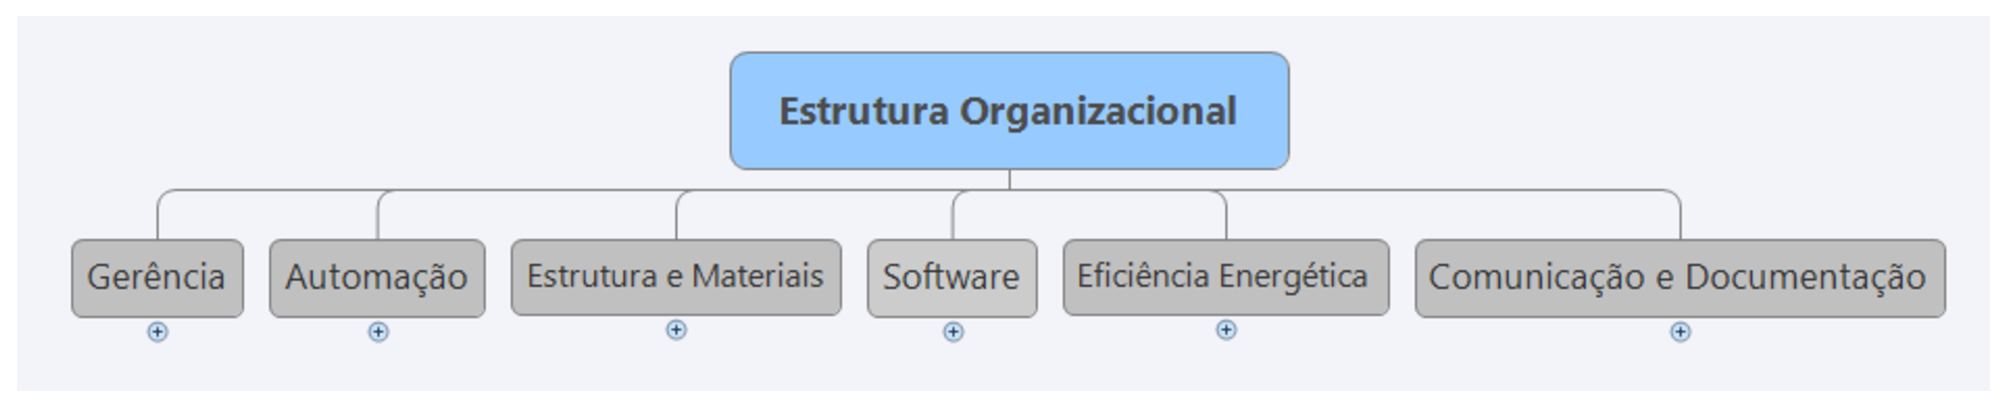
\includegraphics[keepaspectratio,scale=0.5]{figuras/estrutura_organizacional.eps}
	\caption{Estrutura Organizacional}
  \end{center}
\end{figure}

\subsection{Gerência}

	A gerencia é a área que coordenará o andamento do projeto. Cabe a ela impedir empecilhos, evitar atrasos, traçar caminhos alternativos, etc., visando atender a tríplice restrição, tempo, escopo e custo. Se desdobrando em subniveis, os subgerentes são os responsáveis por coordenar cada grupo de conhecimento: automação, estrutura e materiais e eficiência energética.

\subsection{Grupo de Pesquisa}

	A seguir haverá o quadro organizacional dos subgrupos, automação, estrutura e materiais, eficiência energética.

\begin{figure}[H]
  \begin{center}
	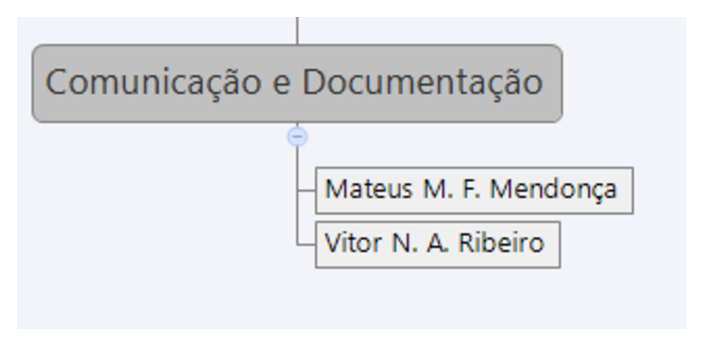
\includegraphics[keepaspectratio,scale=0.6]{figuras/comunicacao_documentacao.eps}
	\caption{Comunicação e Documentação}
  \end{center}
\end{figure}

\begin{figure}[H]
  \begin{center}
	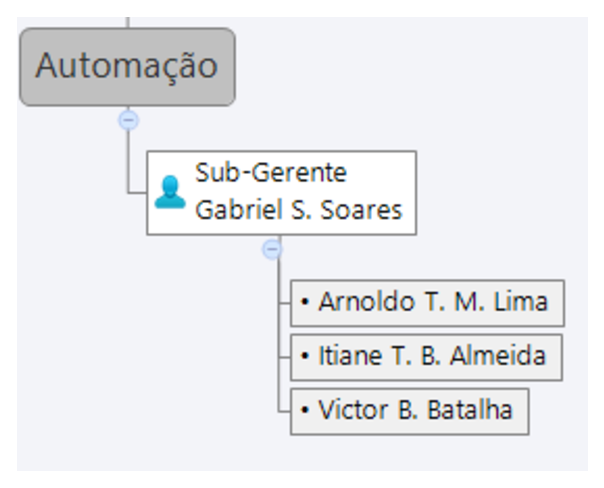
\includegraphics[keepaspectratio,scale=0.6]{figuras/automacao.eps}
	\caption{Automação}
  \end{center}
\end{figure}

\begin{figure}[H]
  \begin{center}
	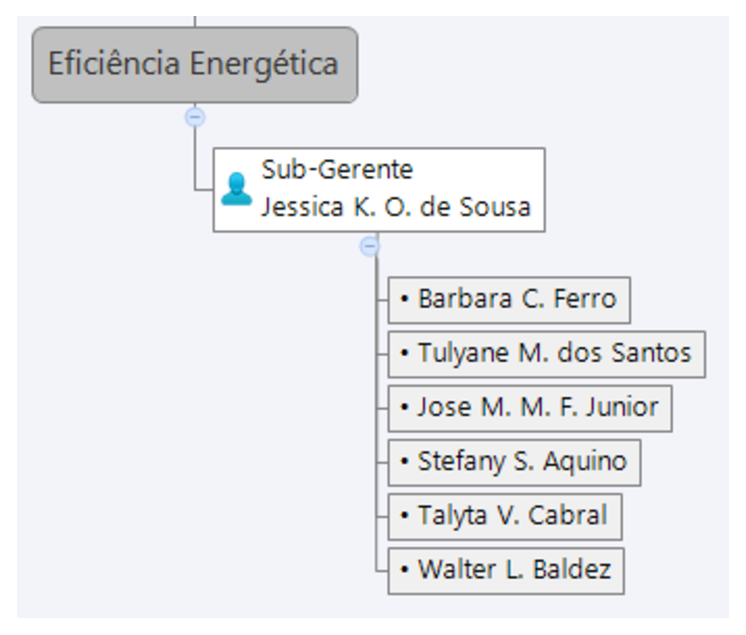
\includegraphics[keepaspectratio,scale=0.6]{figuras/eficiencia_energetica.eps}
	\caption{Eficiência Energética}
  \end{center}
\end{figure}

\begin{figure}[H]
  \begin{center}
	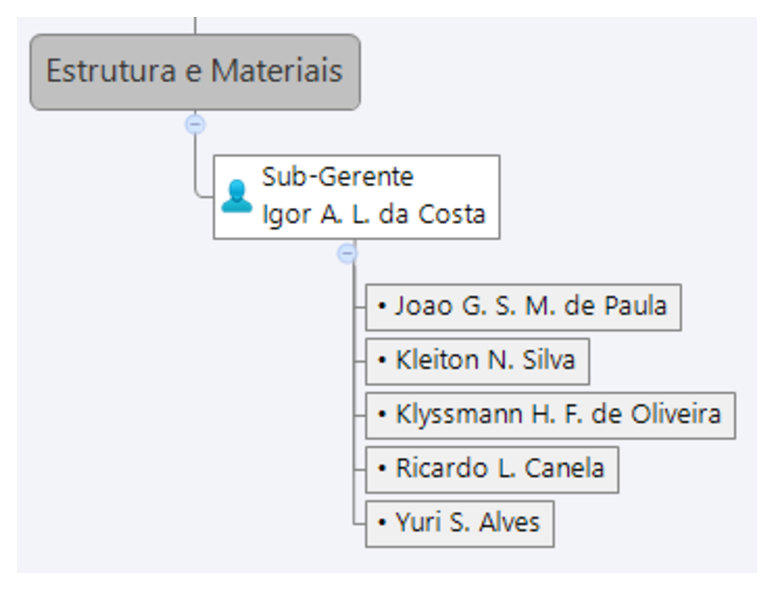
\includegraphics[keepaspectratio,scale=0.6]{figuras/estrutura_materiais.eps}
	\caption{Estrutura e Materiais}
  \end{center}
\end{figure}

\begin{figure}[H]
  \begin{center}
	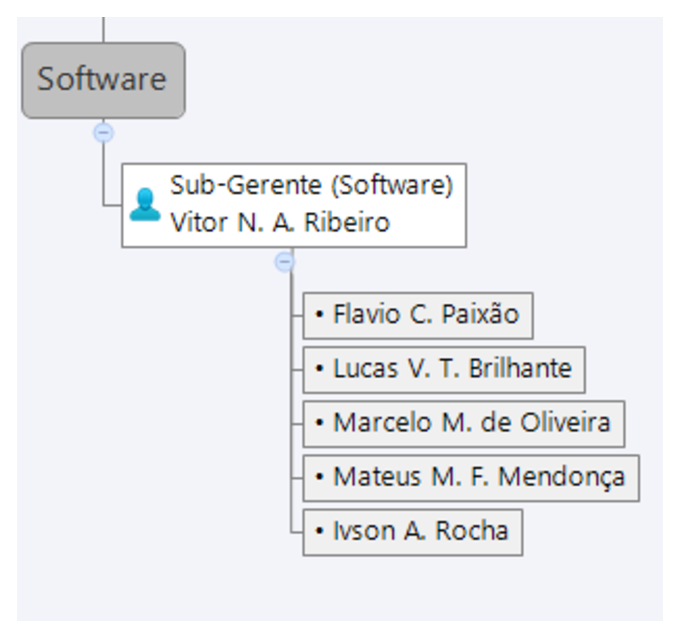
\includegraphics[keepaspectratio,scale=0.6]{figuras/software.eps}
	\caption{Software}
  \end{center}
\end{figure}
